 %\documentclass[wcp,gray]{jmlr} % test grayscale version
 %\documentclass[wcp]{jmlr}% former name JMLR W\&CP
\documentclass[pmlr]{jmlr}% new name PMLR (Proceedings of Machine Learning)

 % The following packages will be automatically loaded:
 % amsmath, amssymb, natbib, graphicx, url, algorithm2e

 %\usepackage{rotating}% for sideways figures and tables
\usepackage{longtable}% for long tables

 % The booktabs package is used by this sample document
 % (it provides \toprule, \midrule and \bottomrule).
 % Remove the next line if you don't require it.
\usepackage{booktabs}
 % The siunitx package is used by this sample document
 % to align numbers in a column by their decimal point.
 % Remove the next line if you don't require it.
\usepackage[load-configurations=version-1]{siunitx} % newer version
 %\usepackage{siunitx}
 
 % to do
 \usepackage{xcolor}
 \newcommand\todo[1]{\textcolor{red}{#1}}

% The following command is just for this sample document:
\newcommand{\cs}[1]{\texttt{\char`\\#1}}

 % Define an unnumbered theorem just for this sample document:
\theorembodyfont{\upshape}
\theoremheaderfont{\scshape}
\theorempostheader{:}
\theoremsep{\newline}
\newtheorem*{note}{Note}

 % change the arguments, as appropriate, in the following:
\jmlrvolume{1}
\jmlryear{2019}
\jmlrworkshop{}


% start article
% \titlebreak
% \footnote{}
% \textsf
% \bfseries

\title[Conformal Prediction for Students' Grades]{Conformal Prediction for Students' Grades in a Course Recommender System\titletag{\thanks{XXX}}}

 % Use \Name{Author Name} to specify the name.
 % If the surname contains spaces, enclose the surname
 % in braces, e.g. \Name{John {Smith Jones}} similarly
 % if the name has a "von" part, e.g \Name{Jane {de Winter}}.
 % If the first letter in the forenames is a diacritic
 % enclose the diacritic in braces, e.g. \Name{{\'E}louise Smith}

 % Authors with different addresses:
  \author{\Name{Rapha\"{e}l Morsomme\nametag{\thanks{with a note}}} \Email{raphael.morsomme@maastrichtuniversity.nl}\\
   \addr Zwingelput 4, 6211 KH Maastricht, the Netherlands	
   \AND
   \Name{Evgueni Smirnov} \Email{smirnov@maastrichtuniversity.nl}\\
   \addr DKE's address, 6211 KH Maastricht, the Netherlands}

 % Three or more authors with the same address:
 % \author{\Name{Author Name1} \Email{an1@sample.com}\\
 %  \Name{Author Name2} \Email{an2@sample.com}\\
 %  \Name{Author Name3} \Email{an3@sample.com}\\
 %  \addr Address}

 % Authors with different addresses:
 % \author{\Name{Author Name1} \Email{abc@sample.com}\\
 % \addr Address 1
 % \AND
 % \Name{Author Name2} \Email{xyz@sample.com}\\
 % \addr Address 2
 %}

% leave editor's section empty?
%\editor{Editor's name}
 % \editors{List of editors' names}

\begin{document}

\maketitle

\begin{abstract}
Course selection can be challenging for student of Liberal Arts programs. In particular, due to the highly personalized curricula of liberal arts students, it is often difficult to assess whether or not a certain course is too advanced given their academic background. To assist students of the liberal arts program of the University College Maastricht, Morsomme and Vazquez (2019) developed a course recommender system that suggests courses whose content matches the student's academic interests, and issues warnings for courses that it deems too advanced. To accomplish the latter, we fit a sparse regression model for grade. In this paper, we use the Inductive Confidence Machine (Papadopoulos, 2002) to obtain predictive regions for future grades. We compare the results obtained with the standard regression nonconformity measure and the normalized nonconformity measure. We find that both nonconformity measures produce valid predictive regions and that the width of the predictive regions is correlated with the accuracy of the regression model.
\end{abstract}

\begin{keywords} Conformal Prediction, Recommender System, Grade Prediction, Lasso, Education \end{keywords}

\todo{Rapha\"{e}l: make all figures black and white}

\todo{question: make flowchart with two pillars (course recommendation and warnings) instead of input/model/intermediate results/output?}

\todo{connect with bibtex bibliography from citavi}

\section{Introduction}
\label{sec:intro}

difficult to assess if student ready. 
Morsomme and Vazquez include warnings based on grade prediction to help student identify course too advanced for them. Provide warning if predicted grade is a fail.

In this paper, we present an applictaion of the ICM to provide students with prediction regions instead of warnings based on a point estimate for the grade. The advantage of PR over point estimates is that it improves info position of student, tehreby enabling them to make better-informed course selection. We decide to use conformal prediction prediction to tailor the PR to the students and to use an ICM to alleviate the computational costs of transductive. 

Liberal Arts program are often characterized by their open curriculum which allows student to tailor their own study program to their academic objectives. These highly personalized curricula make it difficult for students, academic advisors and course coordinators to assess whether a particular course is too advanced given the student's current academic background or whether she/he has acquired the prerequisite skills via a combination of courses. To alleviate this problem, Morsomme and Vazquez (2019) developed a course recommender system which suggest courses whose content matches the academic interests of the student and issues warnings for courses that it deems too advanced given the student's academic background. To accomplish the latter, they fit a sparse regression model to each course which takes as input a model of the student indicating the skills that she/he has acquired in previous courses and her/his academic performance in different academic disciplines in order to predict grades. Warnings are issued when the system predicts a fail grade.



This paper presents the application of an Inductive Confidence Machine (ICM) (Papadopoulos, 2002) to complement the existing course recommender system of [ref: Morsomme and Vazquez, 2019] with predictive regions for future grades tailored to the student.


To improve student info position, we complement point estimates predictions with region predictions. To tailor the prediction to each student, we use conformal prediction.

This way, the information position of students is improved; instead of providing students with a binary advice, i.e. a warning if the predicted grade is a fail and nothing if it is a passing grade, students are provided with a predictive regions indicating a range of grades they are likely to receive in the courses that they are, for instance, considering for the following term particular course.

We present previous research on grade prediction in \sectionref{sec:related} and the data in \sectionref{sec:data}
We introduce the methodology related to the course recommender system and the ICM in \sectionref{sec:methodology} and present the results in \sectionref{sec:results}

\section{Related Work (Evgueni)}
\label{sec:related}

Conclusion of the section: no previous research has applied the conformal prediction framework to students' grade prediction.

\section{Data}
\label{sec:data}

We employ two sets of data: student data and course data.

The student data consists of anonymized course enrollment information. We use the transcripts of the 2,526 students of the liberal arts program between 2008 and 2019 with a total of 79,245 course enrollments. We exclude enrollments with a missing grade which indicates that the student either dropped the course or fail the attendance requirement. In the latter case, the data set contains an observation corresponding to the resit. \tableref{tab:student-data} presents the student data. Each row contains an anonymized student ID, a course ID, a year and semester, and the obtained grade.

The course data consists of the 2018-2019 course catalogues of five departments of Maastricht University: European Studies, University College Maastricht, University College Venlo, Psychology and Science Program. These catalogues contain a one-page description of 490 courses. \tableref{tab:course-data} presents the textual data in the tidy format with one row per document-term [ref: Wickham 2014]. We process the data following common cleaning procedures [ref: Meyer, 2008]: we tokenize the individual terms, stem them with the Hunspell dictionary and remove common stop words, numbers between 1 and 1,000, and terms occurring less than 3 times in the data set.

\begin{table}[hbtp]
	\floatconts
	{tab:student-data}
	{\caption{Example of Student Data}}	
	{\begin{tabular}{ccccc}
		\toprule
		\bfseries Student ID &\bfseries Course ID &\bfseries Academic Year &\bfseries Period &\bfseries Grade\\
		\midrule
		44940 & CAP3000 & 2009-2010 & 4 & 8.8\\
		37490 & SSC2037 & 2009-2010 & 4 & 8.4\\
		71216 & HUM1003 & 2010-2011 & 4 & 6.8\\
		44212 & SSC2049 & 2010-2011 & 2 & 8.4\\
		85930 & SSC2043 & 2011-2012 & 1 & 4.3\\
		\addlinespace
		14492 & COR1004 & 2012-2013 & 2 & 8.5\\
		34750 & HUM2049 & 2013-2014 & 5 & 6.0\\
		32316 & SSC1001 & 2013-2014 & 1 & 8.5\\
		22092 & SCI1009 & 2014-2015 & 1 & 6.4\\
		19512 & COR1004 & 2016-2017 & 5 & 7.0\\
		\bottomrule
	\end{tabular}}	
\end{table}

\begin{table}[hbtp]
	\floatconts
	{tab:course-data}
	{\caption{Example of Course Data}}	
	{\begin{tabular}{cccc}
			\toprule
			\bfseries Course ID &\bfseries Course Title &\bfseries Department &\bfseries Term\\
			\midrule
			HUM3034 & World History & UCM & understand\\
			HUM3034 & World History & UCM & major\\
			HUM3034 & World History & UCM & issue\\
			HUM3034 & World History & UCM & episode\\
			HUM3034 & World History & UCM & shape\\
			\addlinespace
			HUM3034 & World History & UCM & history\\
			HUM3034 & World History & UCM & mankind\\
			HUM3034 & World History & UCM & focus\\
			HUM3034 & World History & UCM & theme\\
			HUM3034 & World History & UCM & topic\\
			\bottomrule
	\end{tabular}}	
\end{table}

\section{Methodology}
\label{sec:methodology}

\subsection{The Course Recommender System}
\label{sec:crs}

\subsubsection{Overview}
\label{sec:overview}
The course recommender system has two goals: suggesting courses whose content matches the student's academic interests and help the student assess whether she/he has acquired the necessary knowledge to succeed in the course she /he is considering for the following term. Although the former is not of direct interest for this paper, we briefly describe 

\begin{figure}[htbp]
	\floatconts
	{fig:flowchart}
	{\caption{Flowchart of the Course Recommender System}}
	{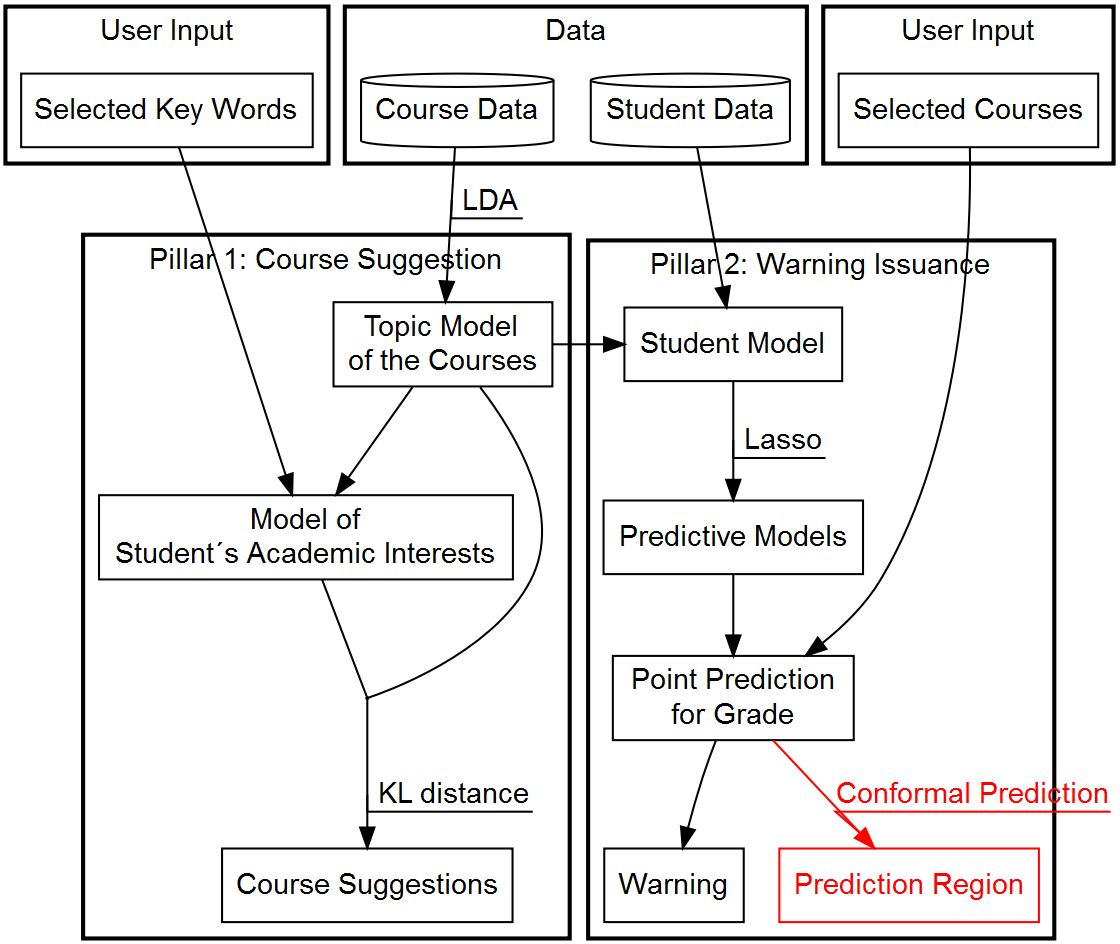
\includegraphics[width=0.5\linewidth]{figures/flowchart}}
\end{figure}

\subsubsection{Topic Model}
\label{sec:tm}
We start by fitting a topic model to the course data using the Latent Dirichlet Allocation generative model and the Gibbs sampling algorithm (ref: Blei, 2003; Phan, 2008). The LDA model views a topic as a mixture of words and a document as a mixture of topics. More precisely, topics are conceptualize as a probability distribution over the vocabulary of the data, and document as a set of words, each drawn from a probability distribution over topics specific to that document. The term \textit{Dirichlet} comes from the fact that the word distribution $\beta_{t}$ for a topic $t$ is generated from a Dirichlet distribution $\beta_{t} \sim Dirichlet(\delta)$ and the topic distribution $\theta_{d}$ for a document $d$ is generated from a Dirichlet distribution $\theta_{d} \sim Dirichlet(\alpha)$ where $\delta$ and $\alpha$ act as hyper-parameters determining how concentrated the distributions of words in topics and the distributions of topics in documents are.

We follow Phan (ref: 2008) who used a Gibbs sampler to learn the distributions $\beta$ and $\theta$. The obtained topic model consists of a term distribution for each topic and a topic distribution for each course description. \figureref{fig:gamma} shows the importance of the main topics of the core course COR1004 Political Philosophy. \figureref{fig:beta} indicates that the two main topics of the course (topics 4 and 19) respectively correspond to the themes of international politics and philosophy.

The number of topics $T$ needs to be specified \textit{a-priori}. We trained 30 models with $K=5,10,\cdots,150$. As suggested by Griffiths and Steyvers (ref: 2008), we set $\alpha=50/K$ and $\delta=0.1$. We run 6,000 iterations of the Gibbs sampler with a burn in of 1,000 iterations and sample every 100 iterations. To prevent being stuck in a local optimum, we use 10 random initialization and keep the best model with respect to the log-likelihood. We choose the number of topics $K$ that yields the model with the maximum likelihood. Figure X shows that the model with 65 topics has the maximum likelihood. To increase the quality of the model, we retrain the model with 16,000 iterations of the the Gibbs sampler, a burn in of 2,000 iterations and 20 random starts and the other parameters at their original values.


\begin{figure}[htbp]
	\floatconts
	{fig:gamma}
	{\caption{Topic Distribution in the course COR1004 Political Philosophy.}}
	{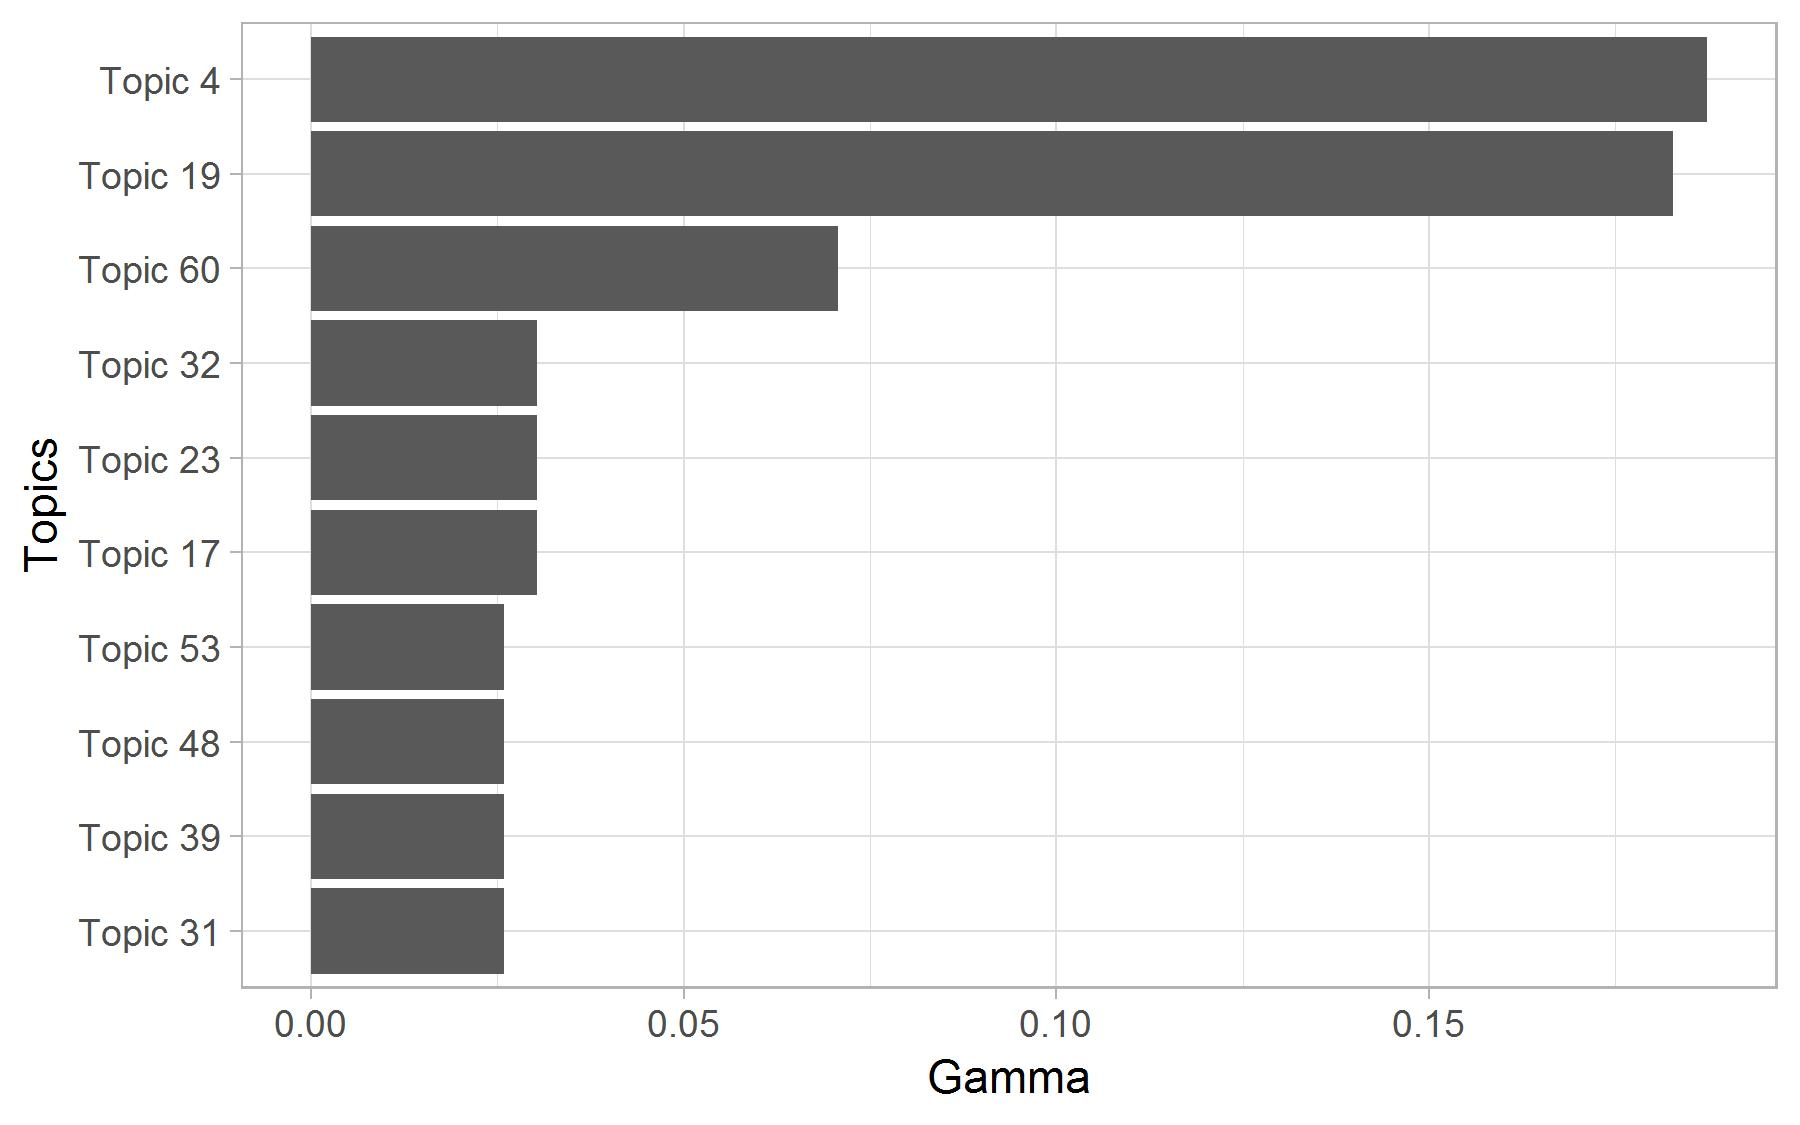
\includegraphics[width=0.5\linewidth]{figures/gamma-COR1004}}
\end{figure}

\begin{figure}[htbp]
	\floatconts
	{fig:beta}
	{\caption{Word Distribution in the main two topics of COR1004 Political Philosophy. Topic 4 corresponds to international politics and Topic 19 to philosophy.}}
	{
		\subfigure[Topic 4]{\label{fig:beta-4}
			\includegraphics[width=0.2\linewidth]{figures/beta-4}}
		\qquad
		\subfigure[Topic 19]{\label{fig:beta-19}%
			\includegraphics[width=0.2\linewidth]{figures/beta-19}}
	}
\end{figure}

\begin{figure}[htbp]
	\floatconts
	{fig:ll}
	{\caption{Maximum Likelihood Model Selection: we choose the model with 65 topics.}}
	{\includegraphics[width=0.5\linewidth]{figures/model-selection}}
\end{figure}

\subsubsection{Student Model}
\label{sec:sm}
The student model consists of two elements: academic performance and level of topic-specific expertise. Academic performance corresponds to the student's general GPA as well as her/his GPA in humanities, natural sciences, social sciences, skills and projects. These are derived from the student's transcript in a straightforward way. Topic-specific expertise corresponds to the knowledge that the student has acquired in each of the topics present in the topic model in previous courses. We posit that when students takes a course they acquire knowledge about its content and that the amount of knowledge they acquire is proportional to their grade. More precisely, we assume that students who obtain 10/10 in a course acquire all the knowledge related to its content and that those who obtain 5/10 only acquire half of it. The content of a course is determined by its topic distribution in the topic model and the grade are retrieved from the student's transcript. Hence if a student has taken $n$ courses and  $g_{i}$ corresponds to her/his grade in  course $i$, for $i = 1, \cdots, n$, then the expertise of the student $e_t$ in topic $t$ simply corresponds to $$e_t = \sum_{i= 1}^{n} g_i \gamma_{i,t}$$ where $\gamma_{i,t}$ corresponds to the importance of topic $t$ in course $i$ in the topic model. \figureref{fig:toy-expertise} presents a toy example of the contribution of individual courses to a student's expertise in 5 topics.


\begin{table}[htbp]
	\floatconts
	{tab:toy}
	{\caption{Toy Example of Topic Expertise}}
	{%
		\subtable[Topic Distribution $\gamma$]{%
			\label{tab:toy-gamma}%
			\begin{tabular}{cccccc}
				\toprule
				\bfseries Course & \bfseries Topic 1 & \bfseries Topic 2 & \bfseries Topic 3 & \bfseries Topic 4 & \bfseries Topic 5\\
				\midrule
				Course 1 & 0.0 & 0.7 & 0.2 & 0.1 & 0.0\\
				Course 2 & 0.2 & 0.2 & 0.2 & 0.2 & 0.2\\
				Course 3 & 0.0 & 0.4 & 0.2 & 0.1 & 0.2\\
				\bottomrule
			\end{tabular}
		}\qquad
		\subtable[Transcript]{%
			\label{tab:toy-grade}%
			\begin{tabular}{cc}
				\toprule
				\bfseries Course & \bfseries Grade\\
				\midrule
				Course 1 & 6/10\\
				Course 2 & 9/10\\
				Course 3 & 2.5/10\\
				\bottomrule
			\end{tabular}
		}\qquad
			\subtable[Course Contribution towards Topic Expertise]{%
			\label{tab:toy-contribution}%
			\begin{tabular}{cccccc}
				\toprule
				\bfseries Course & \bfseries Topic 1 & \bfseries Topic 2 & \bfseries Topic 3 & \bfseries Topic 4 & \bfseries Topic 5\\
				\midrule
				Course 1 & 0.00 & 0.42 & 0.12 & 0.060 & 0.00\\
				Course 2 & 0.18 & 0.18 & 0.18 & 0.180 & 0.18\\
				Course 3 & 0.00 & 0.10 & 0.05 & 0.025 & 0.05\\
				\bottomrule
			\end{tabular}
		}
	}
\end{table}

\begin{figure}[htbp]
	\floatconts
	{fig:toy-expertise}
	{\caption{Contribution of Individual Courses towards a Student's Topic Expertise Profile.}}
	{\includegraphics[width=0.5\linewidth]{figures/toy-expertise}}
\end{figure}



\subsubsection{Underlying Algorithm: Sparse Regression Model}
\label{sec:sm}

We fit a sparse linear regression model for grade prediction to each of the 132 courses currently offered at the college with at least 20 student enrollments since 2008. The input consists of the 71 variables present in the student model at the start of the course: her/his 6 GPA's  (1 general and 5 discipline-specific) and 65 levels of topic-specific expertise. Since the number of predictors is relatively large, we regularize the models with the lasso penalty (ref: Tibshirany, 1998). For each course, we use 10-fold cross-validation to find the value of the lasso tuning parameter $\lambda$ that minimizes the CV mean absolute error (mae), a more robust loss function than the squared absolute error (ref: els, 2008). \figureref{fig:mae-cv} presents the distribution of the CV mae for the 132 prediction models. The model for the course \textit{PRO2004 Academic Debate} has the smallest prediction error (0.38 grade point) and the model for \textit{SCI3006 Mathematical Modelling} the largest (1.80 grade point). The mean CV mae weighted by the number of students enrolled in the course is 0.78, the median is 0.78 and the standard deviation is 0.28.


\begin{figure}[htbp]
	\floatconts
	{fig:cv-mae}
	{\caption{Distribution of Cross-Validation Error}}
	{\includegraphics[width=0.5\linewidth]{figures/cv-mae}}
\end{figure}


\subsubsection{Prediction Region for Grade}
\label{sec:warning}
Import from EDM2019

\subsection{The Inductive Confidence Machine (Evgueni)}
\label{sec:icm}

\section{Results}
\label{sec:results}

Make figures

\section{Conclusion}
\label{sec:conclusion}

valid

width correlated to accuracy of underlying algorithm i.e. CV error of lasso

\section{Comments to Evgueni}

Focus on conformal prediction instead of recommender system, lasso, topic model, etc. This way, the paper is simpler to follow.

If we want to expand on lasso, we should write a paper on lasso itself; just like we are doing with grade prediction. The same goes for topic model.



%%%%%%%%%%%%%%%%%%
%%%%%%%%%%%%%%%%%%


% end of paper


%%%%%%%%%%%%%%%%%%
%%%%%%%%%%%%%%%%%%



\section{others}

This is a sample article that uses the \textsf{jmlr} class with
the \texttt{wcp} class option.  Please follow the guidelines in
this sample document as it can help to reduce complications when
combining the articles into a book. Please avoid using obsolete
commands, such as \verb|\rm|, and obsolete packages, such as
\textsf{epsfig}.\footnote{See
\url{http://www.ctan.org/pkg/l2tabu}}

Please also ensure that your document will compile with PDF\LaTeX.
If you have an error message that's puzzling you, first check for it
at the UK TUG FAQ
\url{http://www.tex.ac.uk/cgi-bin/texfaq2html?label=man-latex}.  If
that doesn't help, create a minimal working example (see
\url{http://theoval.cmp.uea.ac.uk/~nlct/latex/minexample/}) and post
to somewhere like TeX on StackExchange
(\url{http://tex.stackexchange.com/}) or the LaTeX Community Forum
(\url{http://www.latex-community.org/forum/}).

\begin{note}
This is an numbered theorem-like environment that was defined in
this document's preamble.
\end{note}

\subsection{Sub-sections}

Sub-sections are produced using \verb|\subsection|.

\subsubsection{Sub-sub-sections}

Sub-sub-sections are produced using \verb|\subsubsection|.

\paragraph{Sub-sub-sub-sections}

Sub-sub-sub-sections are produced using \verb|\paragraph|.
These are unnumbered with a running head.

\subparagraph{Sub-sub-sub-sub-sections}

Sub-sub-sub-sub-sections are produced using \verb|\subparagraph|.
These are unnumbered with a running head.

\section{Cross-Referencing}

Always use \verb|\label| and \verb|\ref| (or one of the commands
described below) when cross-referencing.  For example, the next
section is Section~\ref{sec:math}. The \textsf{jmlr} class
provides some convenient cross-referencing commands:
\verb|\sectionref|, \verb|\equationref|, \verb|\tableref|,
\verb|\figureref|, \verb|\algorithmref|, \verb|\theoremref|,
\verb|\lemmaref|, \verb|\remarkref|, \verb|\corollaryref|,
\verb|\definitionref|, \verb|\conjectureref|, \verb|\axiomref|,
\verb|\exampleref| and \verb|\appendixref|. The argument of these
commands may either be a single label or a comma-separated list
of labels. Examples:

Referencing sections: \sectionref{sec:math} or
\sectionref{sec:intro,sec:math} or
\sectionref{sec:intro,sec:math,sec:tables,sec:figures}.

Referencing equations: \equationref{eq:trigrule} or
\equationref{eq:trigrule,eq:df} or
\equationref{eq:trigrule,eq:f,eq:df,eq:y}.

Referencing tables: \tableref{tab:operatornames} or
\tableref{tab:operatornames,tab:example} or
\tableref{tab:operatornames,tab:example,tab:example-booktabs}.

Referencing figures: \figureref{fig:nodes} or
\figureref{fig:nodes,fig:teximage} or
\figureref{fig:nodes,fig:teximage,fig:subfigex} or
\figureref{fig:circle,fig:square}.

Referencing algorithms: \algorithmref{alg:gauss} or
\algorithmref{alg:gauss,alg:moore} or
\algorithmref{alg:gauss,alg:moore,alg:net}.

Referencing theorem-like environments: \theoremref{thm:eigenpow},
\lemmaref{lem:sample}, \remarkref{rem:sample}, 
\corollaryref{cor:sample}, \definitionref{def:sample},
\conjectureref{con:sample}, \axiomref{ax:sample} and
\exampleref{ex:sample}.

Referencing appendices: \appendixref{apd:first} or
\appendixref{apd:first,apd:second}.

\section{Equations}
\label{sec:math}

The \textsf{jmlr} class loads the \textsf{amsmath} package, so
you can use any of the commands and environments defined there.
(See the \textsf{amsmath} documentation for further
details.\footnote{Either \texttt{texdoc amsmath} or
\url{http://www.ctan.org/pkg/amsmath}})

Unnumbered single-lined equations should be displayed using
\verb|\[| and \verb|\]|. For example:
\[E = m c^2\]
Numbered single-line equations should be displayed using the
\texttt{equation} environment. For example:
\begin{equation}\label{eq:trigrule}
\cos^2\theta + \sin^2\theta \equiv 1
\end{equation}
This can be referenced using \verb|\label| and \verb|\equationref|.
For example, \equationref{eq:trigrule}.

Multi-lined numbered equations should be displayed using the
\texttt{align} environment.\footnote{For reasons why you 
shouldn't use the obsolete \texttt{eqnarray} environment, see
Lars Madsen, \emph{Avoid eqnarray!} TUGboat 33(1):21--25, 2012.} For example:
\begin{align}
f(x) &= x^2 + x\label{eq:f}\\
f'(x) &= 2x + 1\label{eq:df}
\end{align}
Unnumbered multi-lined equations should be displayed using the
\texttt{align*} environment. For example:
\begin{align*}
f(x) &= (x+1)(x-1)\\
&= x^2 - 1
\end{align*}
If you want to mix numbered with unnumbered lines use the
align environment and suppress unwanted line numbers with
\verb|\nonumber|. For example:
\begin{align}
y &= x^2 + 3x - 2x + 1\nonumber\\
&= x^2 + x + 1\label{eq:y}
\end{align}
An equation that is too long to fit on a single line can be
displayed using the \texttt{split} environment. 
Text can be embedded in an equation using \verb|\text| or
\verb|\intertext| (as used in \theoremref{thm:eigenpow}).
See the \textsf{amsmath} documentation for further details.

\subsection{Operator Names}
\label{sec:op}

Predefined operator names are listed in \tableref{tab:operatornames}.
For additional operators, either use \verb|\operatorname|,
for example $\operatorname{var}(X)$ or declare it with
\verb|\DeclareMathOperator|, for example
\begin{verbatim}
\DeclareMathOperator{\var}{var}
\end{verbatim}
and then use this new command. If you want limits that go above and
below the operator (like \verb|\sum|) use the starred versions
(\verb|\operatorname*| or \verb|\DeclareMathOperator*|).

\begin{table}[htbp]
\floatconts
  {tab:operatornames}%
  {\caption{Predefined Operator Names (taken from 
   \textsf{amsmath} documentation)}}%
  {%
\begin{tabular}{rlrlrlrl}
\cs{arccos} & $\arccos$ &  \cs{deg} & $\deg$ &  \cs{lg} & $\lg$ &  \cs{projlim} & $\projlim$ \\
\cs{arcsin} & $\arcsin$ &  \cs{det} & $\det$ &  \cs{lim} & $\lim$ &  \cs{sec} & $\sec$ \\
\cs{arctan} & $\arctan$ &  \cs{dim} & $\dim$ &  \cs{liminf} & $\liminf$ &  \cs{sin} & $\sin$ \\
\cs{arg} & $\arg$ &  \cs{exp} & $\exp$ &  \cs{limsup} & $\limsup$ &  \cs{sinh} & $\sinh$ \\
\cs{cos} & $\cos$ &  \cs{gcd} & $\gcd$ &  \cs{ln} & $\ln$ &  \cs{sup} & $\sup$ \\
\cs{cosh} & $\cosh$ &  \cs{hom} & $\hom$ &  \cs{log} & $\log$ &  \cs{tan} & $\tan$ \\
\cs{cot} & $\cot$ &  \cs{inf} & $\inf$ &  \cs{max} & $\max$ &  \cs{tanh} & $\tanh$ \\
\cs{coth} & $\coth$ &  \cs{injlim} & $\injlim$ &  \cs{min} & $\min$ \\
\cs{csc} & $\csc$ &  \cs{ker} & $\ker$ &  \cs{Pr} & $\Pr$
\end{tabular}\par
\begin{tabular}{rlrl}
\cs{varlimsup} & $\varlimsup$ 
& \cs{varinjlim} & $\varinjlim$\\
\cs{varliminf} & $\varliminf$ 
& \cs{varprojlim} & $\varprojlim$
\end{tabular}
}
\end{table}

\section{Vectors and Sets}
\label{sec:vec}

Vectors should be typeset using \cs{vec}. For example $\vec{x}$.
The \textsf{jmlr} class also provides \cs{set} to typeset a
set. For example $\set{S}$.

\section{Floats}
\label{sec:floats}

Floats, such as figures, tables and algorithms, are moving
objects and are supposed to float to the nearest convenient
location. Please don't force them to go in a particular place. In
general it's best to use the \texttt{htbp} specifier and don't
put the figure or table in the middle of a paragraph (that is
make sure there's a paragraph break above and below the float).
Floats are supposed to have a little extra space above and below
them to make them stand out from the rest of the text. This extra
spacing is put in automatically and shouldn't need modifying.

To ensure consistency, please \emph{don't} try changing the format of the caption by doing
something like:
\begin{verbatim}
\caption{\textit{A Sample Caption.}}
\end{verbatim}
or
\begin{verbatim}
\caption{\em A Sample Caption.}
\end{verbatim}
You can, of course, change the font for individual words or 
phrases, for example:
\begin{verbatim}
\caption{A Sample Caption With Some \emph{Emphasized Words}.}
\end{verbatim}

\subsection{Tables}
\label{sec:tables}

Tables should go in the \texttt{table} environment. Within this
environment use \verb|\floatconts| (defined by \textsf{jmlr})
to set the caption correctly and center the table contents.

\begin{table}[t]
	
	\caption{\label{tab:}Student Data \label{tab:data-student}}
	\centering
	\begin{tabular}{ccccc}
		\toprule
		Student ID & Course ID & Academic Year & Period & Grade\\
		\midrule
		44940 & CAP3000 & 2009-2010 & 4 & 8.8\\
		37490 & SSC2037 & 2009-2010 & 4 & 8.4\\
		71216 & HUM1003 & 2010-2011 & 4 & 6.8\\
		44212 & SSC2049 & 2010-2011 & 2 & 8.4\\
		85930 & SSC2043 & 2011-2012 & 1 & 4.3\\
		\addlinespace
		14492 & COR1004 & 2012-2013 & 2 & 8.5\\
		34750 & HUM2049 & 2013-2014 & 5 & 6.0\\
		32316 & SSC1001 & 2013-2014 & 1 & 8.5\\
		22092 & SCI1009 & 2014-2015 & 1 & 6.4\\
		19512 & COR1004 & 2016-2017 & 5 & 7.0\\
		\bottomrule
	\end{tabular}
\end{table}

\begin{table}[htbp]
 % The first argument is the label.
 % The caption goes in the second argument, and the table contents
 % go in the third argument.
\floatconts
  {tab:example}%
  {\caption{An Example Table}}%
  {\begin{tabular}{ll}
  \bfseries Dataset & \bfseries Result\\
  Data1 & 0.12345\\
  Data2 & 0.67890\\
  Data3 & 0.54321\\
  Data4 & 0.09876
  \end{tabular}}
\end{table}

If you want horizontal rules you can use the \textsf{booktabs}
package which provides the commands \verb|\toprule|, 
\verb|\midrule| and \verb|\bottomrule|. For example, see
\tableref{tab:example-booktabs}.

\begin{table}[hbtp]
\floatconts
  {tab:example-booktabss}
  {\caption{A Table With Horizontal Lines}}
  {\begin{tabular}{ll}
  \toprule
  \bfseries Dataset & \bfseries Result\\
  \midrule
  Data1 & 0.12345\\
  Data2 & 0.67890\\
  Data3 & 0.54321\\
  Data4 & 0.09876\\
  \bottomrule
  \end{tabular}}
\end{table}

If you want vertical lines as well, you can't use the
\textsf{booktabs} commands as there'll be some unwanted gaps.
Instead you can use \LaTeX's \verb|\hline|, but the rows may
appear a bit cramped.  You can add extra space above or below a
row using \verb|\abovestrut| and \verb|\belowstrut|. For example,
see \tableref{tab:example-hline}.

\begin{table}[htbp]
\floatconts
  {tab:example-hline}
  {\caption{A Table With Horizontal and Vertical Lines}}%
  {%
    \begin{tabular}{|l|l|}
    \hline
    \abovestrut{2.2ex}\bfseries Dataset & \bfseries Result\\\hline
    \abovestrut{2.2ex}Data1 & 0.12345\\
    Data2 & 0.67890\\
    Data3 & 0.54321\\
    \belowstrut{0.2ex}Data4 & 0.09876\\\hline
    \end{tabular}
  }
\end{table}

If you want to align numbers on their decimal point, you can
use the \textsf{siunitx} package. For example, see
\tableref{tab:example-siunitx}. For further details see the
\textsf{siunitx} documentation\footnote{Either \texttt{texdoc
siunitx} or \url{http://www.ctan.org/pkg/siunitx}}.

\begin{table}[htbp]
\floatconts
  {tab:example-siunitx}
  {\caption{A Table With Numbers Aligned on the Decimal Point}}
  {\begin{tabular}{lS[tabformat=3.5]}
  \bfseries Dataset & {\bfseries Result}\\
  Data1 & 0.12345\\
  Data2 & 10.6789\\
  Data3 & 50.543\\
  Data4 & 200.09876
  \end{tabular}}
\end{table}

If the table is too wide, you can adjust the inter-column
spacing by changing the value of \verb|\tabcolsep|. For
example:
\begin{verbatim}
\setlength{\tabcolsep}{3pt}
\end{verbatim}
If the table is very wide but not very long, you can use the
\texttt{sidewaystable} environment defined in the
\textsf{rotating} package (so use \verb|\usepackage{rotating}|).
If the table is too long to fit on a page, you should use the
\texttt{longtable} environment defined in the \textsf{longtable}
package (so use \verb|\usepackage{longtable}|).

\subsection{Figures}
\label{sec:figures}

Figures should go in the \texttt{figure} environment. Within this
environment, use \verb|\floatconts| to correctly position the
caption and center the image. Use \verb|\includegraphics|
for external graphics files but omit the file extension. Do not
use \verb|\epsfig| or \verb|\psfig|. If you want to scale the
image, it's better to use a fraction of the line width rather
than an explicit length. For example, see \figureref{fig:nodes}.

\begin{figure}[htbp]
 % Caption and label go in the first argument and the figure contents
 % go in the second argument
\floatconts
  {fig:nodess}
  {\caption{Example Image}}
  {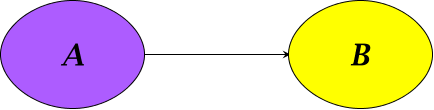
\includegraphics[width=0.5\linewidth]{figures/nodes}}
\end{figure}

If your image is made up of \LaTeX\ code (for example, commands
provided by the \textsf{pgf} package) you can include it using
\cs{includeteximage} (defined by the \textsf{jmlr} class). This
can be scaled and rotated in the same way as \cs{includegraphics}.
For example, see \figureref{fig:teximage}.

\begin{figure}[htbp]
\floatconts
  {fig:teximage}
  {\caption{Image Created Using \LaTeX\ Code}}
  {\includeteximage[angle=45]{figures/teximage}}
\end{figure}

If the figure is too wide to fit on the page, you can use the
\texttt{sidewaysfigure} environment defined in the
\textsf{rotating} package.

Don't use \verb|\graphicspath|. If the figures are contained in
a subdirectory, specify this when you include the image, for
example \verb|\includegraphics{figures/mypic}|.

\subsubsection{Sub-Figures}
\label{sec:subfigures}

Sub-figures can be created using \verb|\subfigure|, which is
defined by the \textsf{jmlr} class. The optional argument allows
you to provide a subcaption. The label should be placed in the
mandatory argument of \verb|\subfigure|. You can reference the
entire figure, for example \figureref{fig:subfigex}, or you can
reference part of the figure using \verb|\figureref|, for example
\figureref{fig:circle}. Alternatively you can reference the
subfigure using \verb|\subfigref|, for example
\subfigref{fig:circle,fig:square} in \figureref{fig:subfigex}.

\begin{figure}[htbp]
\floatconts
  {fig:subfigex}
  {\caption{An Example With Sub-Figures.}}
  {%
    \subfigure[A Circle]{\label{fig:circle}%
      
\includegraphics[width=0.2\linewidth]{figures/circle}}%
    \qquad
    \subfigure[A Square]{\label{fig:square}%
      
\includegraphics[width=0.2\linewidth]{figures/square}}
  }
\end{figure}

By default, the sub-figures are aligned on the baseline.
This can be changed using the second optional argument
of \verb|\subfigure|. This may be \texttt{t} (top), \texttt{c}
(centered) or \texttt{b} (bottom). For example, the subfigures
\subfigref{fig:circle2,fig:square2} in \figureref{fig:subfigex2}
both have \verb|[c]| as the second optional argument.

\begin{figure}[htbp]
\floatconts
  {fig:subfigex2}
  {\caption{Another Example With Sub-Figures.}}
  {%
    \subfigure[A Small Circle][c]{\label{fig:circle2}%
      
\includegraphics[width=0.1\linewidth]{figures/circle}}%
    \qquad
    \subfigure[A Square][c]{\label{fig:square2}%
      
\includegraphics[width=0.2\linewidth]{figures/square}}
  }
\end{figure}

\subsection{Sub-Tables}
\label{sec:subtables}
There is an analogous command \verb|\subtable| for sub-tables.
It has the same syntax as \verb|\subfigure| described above.
You can reference the table using \verb|\tableref|, for example
\tableref{tab:subtabex} or you can reference part of the table,
for example \tableref{tab:ab}. Alternatively you can reference the
subtable using \verb|\subtabref|, for example
\subtabref{tab:ab,tab:cd} in \tableref{tab:subtabex}.

\begin{table}[htbp]
\floatconts
 {tab:subtabex}
 {\caption{An Example With Sub-Tables}}
 {%
   \subtable{%
     \label{tab:ab}%
     \begin{tabular}{cc}
     \bfseries A & \bfseries B\\
     1 & 2
     \end{tabular}
   }\qquad
   \subtable{%
     \label{tab:cd}%
     \begin{tabular}{cc}
     \bfseries C & \bfseries D\\
     3 & 4\\
     5 & 6
     \end{tabular}
   }
 }
\end{table}

By default, the sub-tables are aligned on the top.
This can be changed using the second optional argument
of \verb|\subtable|. This may be \texttt{t} (top), \texttt{c}
(centered) or \texttt{b} (bottom). For example, the sub-tables
\subtabref{tab:ab2,tab:cd2} in \tableref{tab:subtabex2}
both have \verb|[c]| as the second optional argument.

\begin{table}[htbp]
\floatconts
 {tab:subtabex2}
 {\caption{Another Example With Sub-Tables}}
 {%
   \subtable[][c]{%
     \label{tab:ab2}%
     \begin{tabular}{cc}
     \bfseries A & \bfseries B\\
     1 & 2
     \end{tabular}
   }\qquad
   \subtable[][c]{%
     \label{tab:cd2}%
     \begin{tabular}{cc}
     \bfseries C & \bfseries D\\
     3 & 4\\
     5 & 6
     \end{tabular}
   }
 }
\end{table}

\subsection{Algorithms}
\label{sec:algorithms}

Enumerated textual algorithms can be displayed using the
\texttt{algorithm} environment. Within this environment, use
use an \texttt{enumerate} or nested \texttt{enumerate} environments.
For example, see \algorithmref{alg:gauss}. Note that algorithms
float like figures and tables.

\begin{algorithm}[htbp]
\floatconts
{alg:gauss}% label
{\caption{The Gauss-Seidel Algorithm}}
{% contents
\begin{enumerate}
  \item For $k=1$ to maximum number of iterations
    \begin{enumerate}
      \item For $i=1$ to $n$
        \begin{enumerate}
        \item $x_i^{(k)} = 
          \frac{b_i - \sum_{j=1}^{i-1}a_{ij}x_j^{(k)}
          - \sum_{j=i+1}^{n}a_{ij}x_j^{(k-1)}}{a_{ii}}$
        \item If $\|\vec{x}^{(k)}-\vec{x}^{(k-1)} < \epsilon\|$,
          where $\epsilon$ is a specified stopping criteria, stop.
      \end{enumerate}
    \end{enumerate}
\end{enumerate}
}
\end{algorithm}

You can use \verb|\caption| and \verb|\label| without using
\verb|\floatconts| (as in \algorithmref{alg:moore}).

If you'd rather have the same numbering throughout the algorithm
but still want the convenient indentation of nested 
\texttt{enumerate} environments, you can use the
\texttt{enumerate*} environment provided by the \textsf{jmlr}
class. For example, see \algorithmref{alg:moore}.

\begin{algorithm}
\caption{Moore's Shortest Path}\label{alg:moore}
Given a connected graph $G$, where the length of each edge is 1:
\begin{enumerate*}
  \item Set the label of vertex $s$ to 0
  \item Set $i=0$
  \begin{enumerate*}
    \item \label{step:locate}Locate all unlabelled vertices 
          adjacent to a vertex labelled $i$ and label them $i+1$
    \item If vertex $t$ has been labelled,
    \begin{enumerate*}
      \item[] the shortest path can be found by backtracking, and 
      the length is given by the label of $t$.
    \end{enumerate*}
    otherwise
    \begin{enumerate*}
      \item[] increment $i$ and return to step~\ref{step:locate}
    \end{enumerate*}
  \end{enumerate*}
\end{enumerate*}
\end{algorithm}

Pseudo code can be displayed using the \texttt{algorithm2e}
environment. This is defined by the \textsf{algorithm2e} package
(which is automatically loaded) so check the \textsf{algorithm2e}
documentation for further details.\footnote{Either \texttt{texdoc
algorithm2e} or \url{http://www.ctan.org/pkg/algorithm2e}}
For an example, see \algorithmref{alg:net}.

\begin{algorithm2e}
\caption{Computing Net Activation}
\label{alg:net}
 % older versions of algorithm2e have \dontprintsemicolon instead
 % of the following:
 %\DontPrintSemicolon
 % older versions of algorithm2e have \linesnumbered instead of the
 % following:
 %\LinesNumbered
\KwIn{$x_1, \ldots, x_n, w_1, \ldots, w_n$}
\KwOut{$y$, the net activation}
$y\leftarrow 0$\;
\For{$i\leftarrow 1$ \KwTo $n$}{
  $y \leftarrow y + w_i*x_i$\;
}
\end{algorithm2e}

\section{Description Lists}

The \textsf{jmlr} class also provides a description-like 
environment called \texttt{altdescription}. This has an
argument that should be the widest label in the list. Compare:
\begin{description}
\item[add] A method that adds two variables.
\item[differentiate] A method that differentiates a function.
\end{description}
with
\begin{altdescription}{differentiate}
\item[add] A method that adds two variables.
\item[differentiate] A method that differentiates a function.
\end{altdescription}

\section{Theorems, Lemmas etc}
\label{sec:theorems}

The following theorem-like environments are predefined by
the \textsf{jmlr} class: \texttt{theorem}, \texttt{example},
\texttt{lemma}, \texttt{proposition}, \texttt{remark}, 
\texttt{corollary}, \texttt{definition}, \texttt{conjecture}
and \texttt{axiom}. You can use the \texttt{proof} environment
to display the proof if need be, as in \theoremref{thm:eigenpow}.

\begin{theorem}[Eigenvalue Powers]\label{thm:eigenpow}
If $\lambda$ is an eigenvalue of $\vec{B}$ with eigenvector
$\vec{\xi}$, then $\lambda^n$ is an eigenvalue of $\vec{B}^n$
with eigenvector $\vec{\xi}$.
\begin{proof}
Let $\lambda$ be an eigenvalue of $\vec{B}$ with eigenvector
$\xi$, then
\begin{align*}
\vec{B}\vec{\xi} &= \lambda\vec{\xi}
\intertext{premultiply by $\vec{B}$:}
\vec{B}\vec{B}\vec{\xi} &= \vec{B}\lambda\vec{\xi}\\
\Rightarrow \vec{B}^2\vec{\xi} &= \lambda\vec{B}\vec{\xi}\\
&= \lambda\lambda\vec{\xi}\qquad
\text{since }\vec{B}\vec{\xi}=\lambda\vec{\xi}\\
&= \lambda^2\vec{\xi}
\end{align*}
Therefore true for $n=2$. Now assume true for $n=k$:
\begin{align*}
\vec{B}^k\vec{\xi} &= \lambda^k\vec{\xi}
\intertext{premultiply by $\vec{B}$:}
\vec{B}\vec{B}^k\vec{\xi} &= \vec{B}\lambda^k\vec{\xi}\\
\Rightarrow \vec{B}^{k+1}\vec{\xi} &= \lambda^k\vec{B}\vec{\xi}\\
&= \lambda^k\lambda\vec{\xi}\qquad
\text{since }\vec{B}\vec{\xi}=\lambda\vec{\xi}\\
&= \lambda^{k+1}\vec{\xi}
\end{align*}
Therefore true for $n=k+1$. Therefore, by induction, true for all
$n$.
\end{proof}
\end{theorem}

\begin{lemma}[A Sample Lemma]\label{lem:sample}
This is a lemma.
\end{lemma}

\begin{remark}[A Sample Remark]\label{rem:sample}
This is a remark.
\end{remark}

\begin{corollary}[A Sample Corollary]\label{cor:sample}
This is a corollary.
\end{corollary}

\begin{definition}[A Sample Definition]\label{def:sample}
This is a definition.
\end{definition}

\begin{conjecture}[A Sample Conjecture]\label{con:sample}
This is a conjecture.
\end{conjecture}

\begin{axiom}[A Sample Axiom]\label{ax:sample}
This is an axiom.
\end{axiom}

\begin{example}[An Example]\label{ex:sample}
This is an example.
\end{example}

\section{Color vs Grayscale}
\label{sec:color}

It's helpful if authors supply grayscale versions of their
figures in the event that the article is to be incorporated into
a black and white printed book. With external PDF, PNG or JPG
graphic files, you just need to supply a grayscale version of the
file. For example, if the file is called \texttt{myimage.png},
then the gray version should be \texttt{myimage-gray.png} or
\texttt{myimage-gray.pdf} or \texttt{myimage-gray.jpg}. You don't
need to modify your code. The \textsf{jmlr} class checks for
the existence of the grayscale version if it is print mode 
(provided you have used \verb|\includegraphics| and haven't
specified the file extension).

You can use \verb|\ifprint| to determine which mode you are in.
For example, in \figureref{fig:nodes}, the 
\ifprint{dark gray}{purple} ellipse represents an input and the
\ifprint{light gray}{yellow} ellipse represents an output.
Another example: {\ifprint{\bfseries}{\color{red}}important text!}

You can use the class option \texttt{gray} to see how the
document will appear in gray scale mode. \textcolor{blue}{Colored
text} will automatically be converted to gray scale.

The \textsf{jmlr} class loads the \textsf{xcolor}
package, so you can also define your own colors. For example:
\ifprint
  {\definecolor{myred}{gray}{0.5}}%
  {\definecolor{myred}{rgb}{0.5,0,0}}%
\textcolor{myred}{XYZ}.

The \textsf{xcolor} class is loaded with the \texttt{x11names}
option, so you can use any of the x11 predefined colors (listed
in the \textsf{xcolor} documentation\footnote{either 
\texttt{texdoc xcolor} or \url{http://www.ctan.org/pkg/xcolor}}).

\section{Citations and Bibliography}
\label{sec:cite}

The \textsf{jmlr} class automatically loads \textsf{natbib}.
This sample file has the citations defined in the accompanying
BibTeX file \texttt{jmlr-sample.bib}. For a parenthetical
citation use \verb|\citep|. For example
\citep{guyon-elisseeff-03}. For a textual citation use
\verb|\citet|. For example \citet{guyon2007causalreport}.
Both commands may take a comma-separated list, for example
\citet{guyon-elisseeff-03,guyon2007causalreport}.

These commands have optional arguments and have a starred
version. See the \textsf{natbib} documentation for further
details.\footnote{Either \texttt{texdoc natbib} or
\url{http://www.ctan.org/pkg/natbib}}

The bibliography is displayed using \verb|\bibliography|.

\acks{Our thanks to the University College Maastricht, Maastricht University, the Institute of Data Science, and the Department of Data Science and Knowledge Engineering, in particular to Peter Vermeer for initiating the project and enabling collaboration with the University College Maastricht.}

\bibliography{jmlr-sample}

\appendix

\section{First Appendix}\label{apd:first}

This is the first appendix.

\section{Second Appendix}\label{apd:second}

This is the second appendix.

\end{document}
